
\lstdefinelanguage{formula}
   {morekeywords={model,conforms,is,in,uses,domain,partial,transform,from,to,at,extends,includes,new,no,count},
    otherkeywords={:-,:=,::=},
    sensitive=true,
    morecomment=[l]{//},
    morestring=[b]"
   }
 \lstset{
    numbers = none,
    xleftmargin=15pt,
    framexleftmargin=0pt,
    framesep=0pt,
    tabsize=2,
    numbersep=5pt, % how far the line-numbers are from the code
    basicstyle=\footnotesize\ttfamily,
    commentstyle=\normalfont\rmfamily\color{darkgreen},%\bfseries,
    breaklines = true,
    breakatwhitespace = true,
    keywordstyle = \color{FormulaKeywordColor},
    identifierstyle=\color{black},
    language=formula
    }
\chapter{Formal Semantics of AVM Component Model}
\section{Domains}

\subsection{AVM Interchange Format Overview Semantics}
\begin{tabular}{ l l }
\textbf{File} & AVMInterchangeOverview.4ml \\
\textbf{Uses} & AVMInterchange at "AVMInterchange.4ml" \\
\textbf{Extends} &  AVMInterchange \\
\end{tabular}


\subsubsection{Constraints}



\begin{figure}[H]
\centering
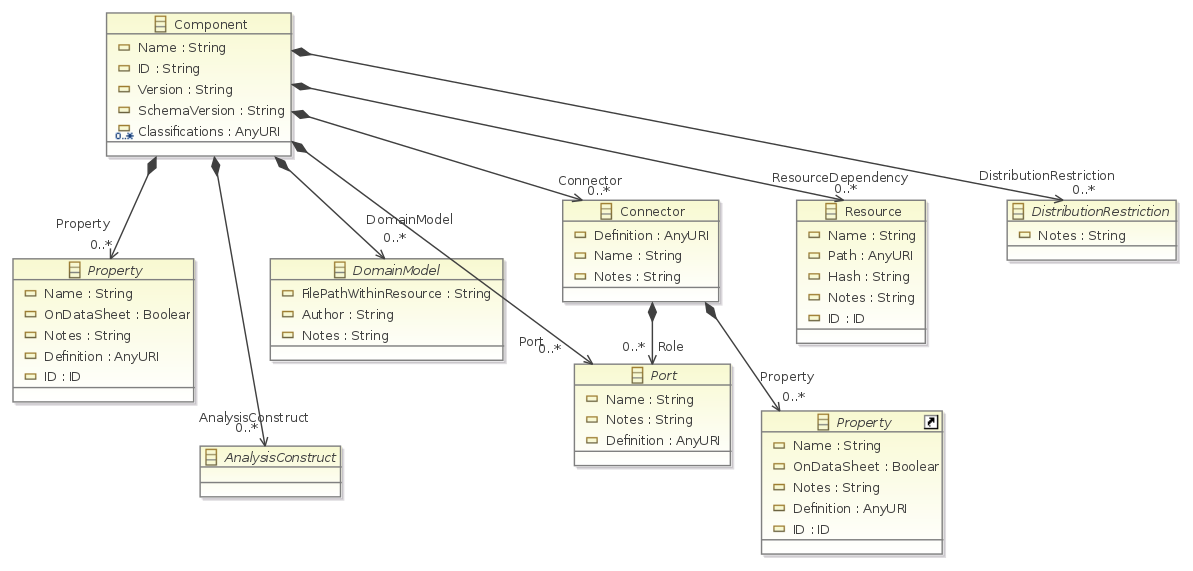
\includegraphics[width=\textwidth]{./AVM_Formal_Semantics/0}
\caption{Component Class Diagram}
\end{figure}

Component Diagram Abstract Types
\begin{lstlisting}

avm_Property ::=
    avm_CompoundProperty +
    avm_PrimitiveProperty.
  avm_AnalysisConstruct ::=
    avm_cad_Geometry +
    avm_cad_CustomGeometry +
    avm_cad_Geometry3D +
    avm_cad_Surface +
    avm_cad_Sphere +
    avm_cad_ExtrudedGeometry +
    avm_cad_Geometry2D +
    avm_cad_Polygon +
    avm_cad_Circle.
  avm_DomainModel ::=
    avm_simulink_SimulinkModel +
    avm_manufacturing_ManufacturingModel +
    avm_cad_CADModel +
    avm_modelica_ModelicaModel.
  avm_Port ::=
    avm_DomainModelPort +
    avm_simulink_Port1 +
    avm_simulink_Signal +
    avm_simulink_OutputSignal +
    avm_simulink_InputSignal +
    avm_AbstractPort +
    avm_cad_Datum +
    avm_cad_CoordinateSystem +
    avm_cad_Plane +
    avm_cad_Axis +
    avm_cad_Point +
    avm_modelica_Connector.
  avm_DistributionRestriction ::=
    avm_ITAR +
    avm_Proprietary +
    avm_SecurityClassification.


\end{lstlisting}

Component Diagram Concrete Types
\begin{lstlisting}

avm_Component ::= new (
    aObjectId: Integer,
    ID: String,
    Name: String,
    SchemaVersion: String,
    Version: String
  ).
  avm_Connector ::= new (
    aObjectId: Integer,
    Definition: String,
    ID: String,
    Name: String,
    Notes: String
  ).
  avm_Resource ::= new (
    aObjectId: Integer,
    Hash: String,
    ID: String,
    Name: String,
    Notes: String,
    Path : String
  ).


\end{lstlisting}

Component Diagram Relationships
\begin{lstlisting}

avm_Component2Property ::= new (
    Property: avm_Component,
    Dst: avm_Property
  ).
  avm_AnalysisConstruct2Component ::= new (
    Src: avm_AnalysisConstruct,
    AnalysisConstruct: avm_Component
  ).
  avm_Component2DomainModel ::= new (
    DomainModel: avm_Component,
    Dst: avm_DomainModel).
  avm_Component2Port ::= new (
    Port: avm_Component,
    Dst: avm_Port
  ).
  avm_Component2Connector ::= new (
    Connector: avm_Component,
    Dst: avm_Connector
  ).
  avm_Component2Resource ::= new (
    ResourceDependency: avm_Component,
    Dst: avm_Resource
  ).
  avm_Component2DistributionRestriction ::= new (
    DistributionRestriction: avm_Component,
    Dst: avm_DistributionRestriction
  ).
  avm_Connector2Port ::= new (
    Role: avm_Connector,
    Dst: avm_Port
  ).
  avm_Connector2Property ::= new (
    Property: avm_Connector,
    Dst: avm_Property
  ).


\end{lstlisting}


\begin{figure}[H]
\centering
\includegraphics[width=\textwidth]{./AVM_Formal_Semantics/1}
\caption{Property Class Diagram}
\end{figure}

Property Diagram Concrete Types
\begin{lstlisting}

avm_CompoundProperty ::= new (
    aObjectId: Integer,
    Definition: String,
    ID: String,
    Name: String,
    Notes: String,
    OnDataSheet: Boolean,
    OnDataSheetSpecified: Boolean
  ).
  avm_PrimitiveProperty ::= new (
    aObjectId: Integer,
    Definition: String,
    ID: String,
    Name: String,
    Notes: String,
    OnDataSheet: Boolean,
    OnDataSheetSpecified: Boolean
  ).
  avm_Value ::= new (
    aObjectId: Integer,
    DataType: DataTypeEnum,
    DataTypeSpecified: Boolean,
    Dimensions: String,
    DimensionType: DimensionTypeEnum,
    DimensionTypeSpecified: Boolean,
    ID: String,
    Unit: String
  ).


\end{lstlisting}

Property Diagram Relationships
\begin{lstlisting}

avm_PrimitiveProperty2Value ::= new (
    Value: avm_PrimitiveProperty,
    Dst: avm_Value
  ).
  avm_CompoundProperty2PrimitiveProperty ::= new (
    PrimitiveProperty: avm_CompoundProperty,
    Dst: avm_PrimitiveProperty
  ).
  avm_CompoundProperty2CompoundProperty ::= new (
    CompoundProperty1: avm_CompoundProperty,
    Dst: avm_CompoundProperty
  ).


\end{lstlisting}


\begin{figure}[H]
\centering
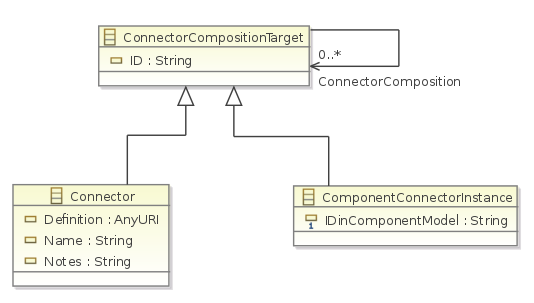
\includegraphics[width=\textwidth]{./AVM_Formal_Semantics/2}
\caption{Connector Class Diagram}
\end{figure}

Connector Diagram Concrete Types
\begin{lstlisting}

avm_ConnectorCompositionTarget ::= new (
    aObjectId: Integer,
    ID: String
  ).
  avm_ComponentConnectorInstance ::= new (
    aObjectId: Integer,
    ID: String,
    IDinComponentModel: String
  ).


\end{lstlisting}

Connector Diagram Relationships
\begin{lstlisting}

avm_ConnectorCompositionTarget2StringSrc ::=
    avm_ConnectorCompositionTarget +
    avm_Connector +
    avm_ComponentConnectorInstance.
  avm_ConnectorCompositionTarget2String ::= new (
    ConnectorComposition: avm_ConnectorCompositionTarget2StringSrc,
    Dst: String //ID of a ConnectorCompositionTarget
  ).


\end{lstlisting}


\begin{figure}[H]
\centering

\includegraphics[width=\textwidth]{./AVM_Formal_Semantics/3}
\caption{Value Interchange Class Diagram}
\end{figure}

Value Diagram Enumerated Types
\begin{lstlisting}

CalculationTypeEnum ::= {
    "Declarative",
    "Python"
  }.
  DataTypeEnum ::= {
    "String",
    "Boolean",
    "Integer",
    "Real"
  }.
  DimensionTypeEnum ::= {
    "Matrix",
    "Vector",
    "Scalar"
  }.


\end{lstlisting}

Value Diagram Abstract Types
\begin{lstlisting}

avm_ValueExpressionType ::=
    avm_ParametricEnumeratedValue +
    avm_FixedValue +
    avm_ProbabilisticValue +
    avm_UniformDistribution +
    avm_NormalDistribution +
    avm_ParametricValue +
    avm_DerivedValue +
    avm_CalculatedValue.
  avm_ProbabilisticValue ::=
    avm_UniformDistribution +
    avm_NormalDistribution.


\end{lstlisting}

Value Diagram Concrete Types
\begin{lstlisting}

avm_DataSource ::= new (
    aObjectId: Integer,
    Notes: String
  ).
  avm_FixedValue ::= new (
    aObjectId: Integer,
    Uncertainty: Real,
    UncertaintySpecified: Boolean,
    Value: String
  ).
  avm_CalculatedValue ::= new (
    aObjectId: Integer,
    Expression: String,
    Type: CalculationTypeEnum
  ).
  avm_DerivedValue ::= new (
    aObjectId: Integer,
    ValueSource: String //Encodes relationship with Value, refers to ID attribute
  ).
  avm_ParametricValue ::= new (
    aObjectId: Integer
  ).
  avm_ParametricEnumeratedValue ::= new (
    aObjectId: Integer
  ).
  avm_UniformDistribution ::= new (
    aObjectId: Integer
  ).
  avm_NormalDistribution ::= new (
    aObjectId: Integer
  ).


\end{lstlisting}

Value Diagram Relationships
\begin{lstlisting}

avm_Value2ValueExpressionType ::= new (
    ValueExpression: avm_Value,
    Dst: avm_ValueExpressionType
  ).
  avm_ParametricValue2ValueExpressionType ::= new (
    Default: avm_ParametricValue,
    Dst: avm_ValueExpressionType //Default
  ).
  avm_ParametricValue2ValueExpressionType1 ::= new (
    Maximum: avm_ParametricValue,
    Dst: avm_ValueExpressionType //Maximum
  ).
  avm_ParametricValue2ValueExpressionType2 ::= new (
    Minimum: avm_ParametricValue,
    Dst: avm_ValueExpressionType //Minimum
  ).
  avm_ParametricValue2ValueExpressionType3 ::= new (
    AssignedValue: avm_ParametricValue,
    Dst: avm_ValueExpressionType //AssignedValue
  ).
  avm_DataSource2Value ::= new (
    Src: avm_DataSource,
    DataSource: avm_Value
  ).
  avm_DataSource2String ::= new (
    FromResource: avm_DataSource,
    Dst: String //ID of Resource
  ).
  avm_FixedValue2ParametricEnumeratedValue ::= new (
    Src: avm_FixedValue,
    AssignedValue: avm_ParametricEnumeratedValue
  ).
  avm_ParametricEnumeratedValue2ValueExpressionType ::= new (
    Enum: avm_ParametricEnumeratedValue,
    Dst: avm_ValueExpressionType
  ).
  avm_NormalDistribution2ValueExpressionType ::= new (
    Mean: avm_NormalDistribution,
    Dst: avm_ValueExpressionType //Mean
  ).
  avm_NormalDistribution2ValueExpressionType1 ::= new (
    StandardDeviation: avm_NormalDistribution,
    Dst: avm_ValueExpressionType //StandardDeviation
  ).


\end{lstlisting}


\begin{figure}[H]
\centering
\includegraphics[width=\textwidth]{./AVM_Formal_Semantics/4}
\caption{Domain Model Class Diagram}
\end{figure}

TODO: Add description of domain model diagram

\begin{figure}[H]
\centering

\includegraphics[width=\textwidth]{./AVM_Formal_Semantics/5}
\caption{Design Interchange Class Diagram}
\end{figure}

Design Diagram Abstract Types
\begin{lstlisting}

avm_Container ::=
    avm_DesignSpaceContainer +
    avm_Alternative +
    avm_Optional +
    avm_Compound.
  avm_DesignSpaceContainer ::=
    avm_Alternative +
    avm_Optional.


\end{lstlisting}

Design Diagram Concrete Types
\begin{lstlisting}

avm_Design ::= new (
    aObjectId: Integer,
    DesignID: String,
    Name: String
  ).
  avm_Compound ::= new (
    aObjectId: Integer,
    Name: String
  ).
  avm_Alternative ::= new (
    aObjectId: Integer,
    Name: String
  ).
  avm_Optional ::= new (
    aObjectId: Integer,
    Name: String
  ).
  avm_ComponentInstance ::= new (
    aObjectId: Integer,
    ComponentID: String,
    ID: String,
    Name: String
  ).
  avm_ComponentPortInstance ::= new (
    aObjectId: Integer,
    ID: String,
    IDinComponentModel: String
  ).
  avm_ComponentPrimitivePropertyInstance ::= new (
    aObjectId: Integer,
    IDinComponentModel: String
  ).


\end{lstlisting}

Design Diagram Relationships
\begin{lstlisting}

avm_Container2Design ::= new (
    Src: avm_Container,
    RootContainer: avm_Design
  ).
  avm_Container2Port ::= new (
    Port: avm_Container,
    Dst: avm_Port
  ).
  avm_Container2Property ::= new (
    Property: avm_Container,
    Dst: avm_Property
  ).
  avm_Connector2Container ::= new (
    Src: avm_Connector,
    Connector: avm_Container
  ).
  avm_Container2Container ::= new (
    Container1: avm_Container,
    Dst: avm_Container
  ).
  avm_ComponentInstance2Container ::= new (
    Src: avm_ComponentInstance,
    ComponentInstance: avm_Container
  ).
  avm_ComponentInstance2ComponentPortInstance ::= new (
    PortInstance: avm_ComponentInstance,
    Dst: avm_ComponentPortInstance
  ).
  avm_ComponentInstance2ComponentPrimitivePropertyInstance ::= new (
    PrimitivePropertyInstance: avm_ComponentInstance,
    Dst: avm_ComponentPrimitivePropertyInstance
  ).
  avm_ComponentConnectorInstance2ComponentInstance ::= new (
    Src: avm_ComponentConnectorInstance,
    ConnectorInstance: avm_ComponentInstance
  ).


\end{lstlisting}


\begin{figure}[H]
\centering

\includegraphics[width=\textwidth]{./AVM_Formal_Semantics/6}
\caption{Port Class Diagram}
\end{figure}

Port Diagram Elements
\begin{lstlisting}

avm_DomainModelPort ::=
    avm_simulink_Port1 +
    avm_simulink_Signal +
    avm_simulink_OutputSignal +
    avm_simulink_InputSignal +
    avm_cad_Datum +
    avm_cad_CoordinateSystem +
    avm_cad_Plane +
    avm_cad_Axis +
    avm_cad_Point +
    avm_modelica_Connector.
  avm_PortMapTarget ::= new (
    aObjectId: Integer,
    ID: String
  ).
  avm_AbstractPort ::= new (
    aObjectId: Integer,
    Definition: String,
    ID: String,
    Name: String,
    Notes: String
  ).
  avm_PortMapTarget2StringSrc ::=
    avm_PortMapTarget +
    avm_AbstractPort +
    avm_ComponentPortInstance +
    avm_cad_Point +
    avm_cad_Axis +
    avm_cad_Plane +
    avm_cad_CoordinateSystem +
    avm_modelica_Connector +
    avm_simulink_InputSignal +
    avm_simulink_OutputSignal.
  avm_PortMapTarget2String ::= new (
    PortMap: avm_PortMapTarget2StringSrc,
    Dst: String //ID of the other PortMapTarget
  ).


\end{lstlisting}


\begin{figure}[H]
\centering
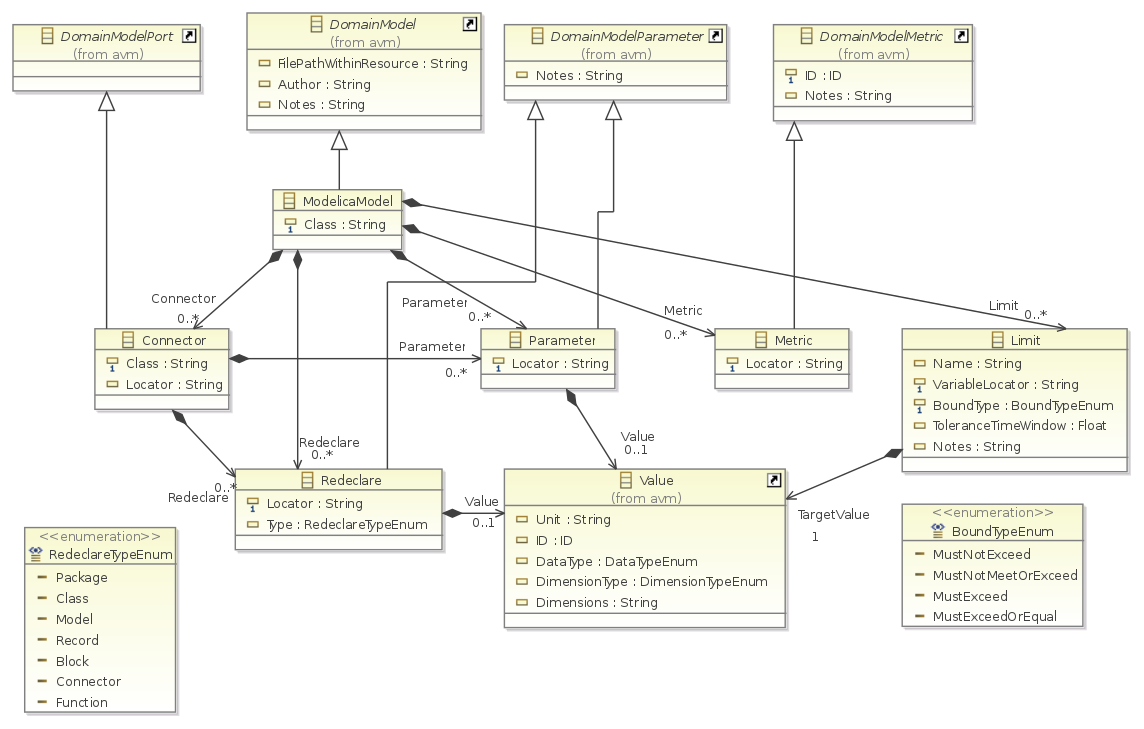
\includegraphics[width=\textwidth]{./AVM_Formal_Semantics/7}
\caption{Modelica Domain Model Class Diagram}
\end{figure}

Modelica Diagram Elements
\begin{lstlisting}

RedeclareTypeEnum ::= {
    "Package",
    "Class",
    "Model",
    "Record",
    "Block",
    "Connector",
    "Function"
  }.
  BoundTypeEnum ::= {
    "MustNotExceed",
    "MustNotMeetOrExceed",
    "MustExceed",
    "MustExceedOrEqual"
  }.
  avm_modelica_ModelicaModel ::= new (
    aObjectId: Integer, 
    Author: String,
    Class: String,
    FilePathWithinResource: String,
    Notes: String,
    UsesResource: String).
  avm_modelica_Connector ::= new (
    aObjectId: Integer,
    Class: String,
    Definition: String,
    ID: String,
    Locator: String,
    Name: String,
    Notes: String
  ).
  avm_modelica_Parameter ::= new (
    aObjectId: Integer,
    Locator: String,
    Notes: String
  ).
  avm_modelica_Metric ::= new (
    aObjectId: Integer,
    ID: String,
    Locator: String,
    Notes: String
  ).
  avm_modelica_Limit ::= new (
    aObjectId: Integer,
    BoundType: BoundTypeEnum,
    Name: String,
    Notes: String,
    ToleranceTimeWindow: Real,
    ToleranceTimeWindowSpecified: Boolean,
    VariableLocator: String
  ).
  avm_modelica_Redeclare ::= new (
    aObjectId: Integer,
    Locator: String,
    Notes: String,
    Type: RedeclareTypeEnum,
    TypeSpecified: Boolean
  ).
  avm_modelica_Connector2ModelicaModel ::= new (
    Src: avm_modelica_Connector,
    Connector: avm_modelica_ModelicaModel
  ).
  avm_modelica_ModelicaModel2Redeclare ::= new (
    Redeclare: avm_modelica_ModelicaModel,
    Dst: avm_modelica_Redeclare
  ).
  avm_modelica_ModelicaModel2Parameter ::= new (
    Parameter: avm_modelica_ModelicaModel,
    Dst: avm_modelica_Parameter
  ).
  avm_modelica_Metric2ModelicaModel ::= new (
    Src: avm_modelica_Metric,
    Metric: avm_modelica_ModelicaModel
  ).
  avm_modelica_Limit2ModelicaModel ::= new (
    Src: avm_modelica_Limit,
    Limit: avm_modelica_ModelicaModel
  ).
  avm_modelica_Connector2Parameter ::= new (
    Parameter: avm_modelica_Connector,
    Dst: avm_modelica_Parameter
  ).
  avm_modelica_Connector2Redeclare ::= new (
    Redeclare: avm_modelica_Connector,
    Dst: avm_modelica_Redeclare
  ).
  avm_modelica_Redeclare2Value ::= new (
    Value: avm_modelica_Redeclare,
    Dst: avm_Value
  ).
  avm_modelica_Parameter2Value ::= new (
    Value: avm_modelica_Parameter,
    Dst: avm_Value
  ).
  avm_modelica_Limit2Value ::= new (
    TargetValue: avm_modelica_Limit,
    Dst: avm_Value
  ).

\end{lstlisting}


\subsection{AVM Interchange Format Structural Semantics}
\begin{tabular}{ l l }
\textbf{File} & AVMInterchangeStructural.4ml \\
\textbf{Uses} & AVMInterchange at "AVMInterchange.4ml" \\
\textbf{Extends} &  AVMInterchange \\
\end{tabular}


\subsubsection{Constraints}


Reference relationships in the interchange format are handled by relating the source object ot the ID of its target.These relations are invalid if there is no object of the appropriate type with the referenced ID.
\begin{lstlisting}

InvalidIDRef :-
    avm_cad_PlaneReference2String(_, id), no avm_cad_Plane(_, _, _, id, _, _);
    avm_ConnectorCompositionTarget2String(_, id), no avm_ConnectorCompositionTarget(_, id), no avm_Connector(_, _, id, _, _), no avm_ComponentConnectorInstance(_, id, _);
    avm_PortMapTarget2String(_, id), id != "", no avm_AbstractPort(_, _, id, _, _), no avm_cad_Axis(_, _, _, id, _, _), no avm_cad_CoordinateSystem(_, _, _, id, _, _), no avm_cad_Plane(_, _, _, id, _, _), no avm_modelica_Connector(_, _, _, id, _, _, _), no avm_ComponentPortInstance(_, id, _);
    avm_DerivedValue(_, id), no avm_Value(_, _, _, _, _, _, id, _).


\end{lstlisting}

The ComponentID attribute of an avm.ComponentInstance must refer to an existing avm.Component.
\begin{lstlisting}

ComponentInstanceInvalidComponentID :-
    avm_ComponentInstance(_, compID, _, _), no avm_Component(_, compID, _, _, _).

\end{lstlisting}


\subsection{Helper Rules for Interchange Domain}
\begin{tabular}{ l l }
\textbf{File} & AVMInterchangeHelpful.4ml \\
\textbf{Uses} & AVMInterchange at "AVMInterchange.4ml" \\
\textbf{Extends} &  AVMInterchange \\
\end{tabular}


\subsubsection{Constraints}


The AVMInterchangeHelpful domain extends the original generated AVMInterchange domain with severalrules for aggregation (e.g. of the notion of containment) and simplification.
Relates and ID-possessing element from the interchange domain to its ID.
\begin{lstlisting}

HasID ::= (AVMInterchange.Data, String).
  HasID(obj, id) :-
    obj is avm_PortMapTarget(_, id);
    obj is avm_simulink_OutputSignal(_, _, _, id, _, _, _);
    obj is avm_simulink_InputSignal(_, _, _, id, _, _, _);
    obj is avm_Component(_, id, _, _, _);
    obj is avm_ComponentPortInstance(_, id, _);
    obj is avm_AbstractPort(_, _, id, _, _);
    obj is avm_ConnectorCompositionTarget(_, id);
    obj is avm_ComponentConnectorInstance(_, id, _);
    obj is avm_Connector(_, _, id, _, _);
    obj is avm_CompoundProperty(_, _, id, _, _, _, _);
    obj is avm_PrimitiveProperty(_, _, id, _, _, _, _);
    obj is avm_Value(_, _, _, _, _, _, id, _);
    obj is avm_Resource(_, _, id, _, _, _);
    obj is avm_ComponentInstance(_, _, id, _);
    obj is avm_manufacturing_Metric(_, id, _, _);
    obj is avm_cad_Metric(_, id, _, _);
    obj is avm_cad_CoordinateSystem(_, _, _, id, _, _);
    obj is avm_cad_Plane(_, _, _, id, _, _);
    obj is avm_cad_Axis(_, _, _, id, _, _);
    obj is avm_cad_Point(_, _, _, id, _, _);
    obj is avm_modelica_Metric(_, id, _, _);
    obj is avm_modelica_Connector(_, _, _, id, _, _, _).


\end{lstlisting}

Serves as a polymorphic accessor for avm\_Container concrete subtypes and converts their respective typesinto a string, which corresponds to the way it is represented in CyPhyML.
\begin{lstlisting}

AVMDesignContainer ::= (container:avm_Container, aObjectID:Integer, Name:String, Type:String).
  AVMDesignContainer(cont, aID, name, type) :-
    cont is avm_Compound(aID, name), type = "Compound";
    cont is avm_Alternative(aID, name), type = "Alternative";
    cont is avm_Optional(aID, name), type = "Optional".


\end{lstlisting}

Serves as a polymorphic accessor for avm\_Port concrete subtypes.
\begin{lstlisting}

AVMPort ::= (port:avm_Port, aObjectID:Integer, ID:String, Name:String, Notes:String, Definition:String).
  AVMPort(port, aID, id, name, notes, def) :-
    port is avm_AbstractPort(aID, def, id, name, notes);
    port is avm_modelica_Connector(aID, _, def, id, _, name, notes);
    port is avm_cad_Axis(aID, _, def, id, name, notes);
    port is avm_cad_Point(aID, _, def, id, name, notes);
    port is avm_cad_Plane(aID, _, def, id, name, notes);
    port is avm_cad_CoordinateSystem(aID, _, def, id, name, notes);
    port is avm_simulink_InputSignal(aID, _, def, id, _, name, notes);
    port is avm_simulink_OutputSignal(aID, _, def, id, _, name, notes).


\end{lstlisting}

Aggregates all containment relationships from the Interchange domain into a single easy to use andunderstand 'Contains' relationship.
\begin{lstlisting}

Contains ::= (AVMInterchange.Data, AVMInterchange.Data).
  Contains(a, b) :-
    avm_cad_ExtrudedGeometry2Geometry2D(a, b);
    avm_cad_CustomGeometryInput2Geometry(a, b);
    avm_cad_CustomGeometry2CustomGeometryInput(a, b);
    avm_cad_Circle2PointReference(a, b); //Circle -> CircleCenter
    avm_cad_Circle2PointReference1(a, b); //Circle -> CircleEdge
    avm_cad_PointReference2Polygon(b, a);
    avm_cad_ExtrudedGeometry2PointReference(a, b);
    avm_cad_PointReference2Sphere(b, a); //SphereCenter <- Sphere
    avm_cad_PointReference2Sphere1(b, a); //SphereEdge <- Sphere
    avm_cad_PlaneReference2Surface(b, a);
    avm_cad_CADModel2Metric(a, b);
    avm_cad_CADModel2Parameter(a, b);
    avm_cad_CADModel2Datum(a, b);
    avm_cad_Datum2Metric(a, b);
    avm_cad_Parameter2Value(a, b);
    avm_Component2Property(a, b);
    avm_AnalysisConstruct2Component(b, a);
    avm_Component2DomainModel(a, b);
    avm_Component2Connector(a, b);
    avm_Component2Port(a, b);
    avm_Component2Resource(a, b);
    avm_Component2DistributionRestriction(a, b);
    avm_Connector2Port(a, b);
    avm_Connector2Property(a, b);
    avm_Container2Container(a, b);
    avm_Container2Design(b, a);
    avm_Container2Property(a, b);
    avm_Container2Port(a, b);
    avm_Connector2Container(b, a);
    avm_ComponentInstance2ComponentPortInstance(a, b);
    avm_ComponentInstance2ComponentPrimitivePropertyInstance(a, b);
    avm_ComponentConnectorInstance2ComponentInstance(b, a);
    avm_ComponentInstance2Container(b, a);
    avm_ComponentPrimitivePropertyInstance2Value(a, b);
    avm_DomainModelMetric2Value(a, b);
    avm_manufacturing_ManufacturingModel2Metric(a, b);
    avm_manufacturing_ManufacturingModel2Parameter(a, b);
    avm_manufacturing_Parameter2Value(a, b);
    avm_modelica_Connector2ModelicaModel(b, a);
    avm_modelica_ModelicaModel2Redeclare(a, b);
    avm_modelica_ModelicaModel2Parameter(a, b);
    avm_modelica_Metric2ModelicaModel(b, a);
    avm_modelica_Limit2ModelicaModel(b, a);
    avm_modelica_Connector2Redeclare(a, b);
    avm_modelica_Connector2Parameter(a, b);
    avm_modelica_Parameter2Value(a, b);
    avm_modelica_Limit2Value(b, a);
    avm_CompoundProperty2CompoundProperty(b, a);
    avm_CompoundProperty2PrimitiveProperty(a, b);
    avm_PrimitiveProperty2Value(a, b);
    avm_simulink_Port12SimulinkModel(b, a);
    avm_simulink_Parameter2SimulinkModel(b, a);
    avm_simulink_Parameter2Value(a, b);
    avm_DataSource2Value(b, a);
    avm_Value2ValueExpressionType(a, b);
    avm_ParametricValue2ValueExpressionType(a, b); //ParametricValue -> Default
    avm_ParametricValue2ValueExpressionType1(a, b); //ParametricValue -> Maximum
    avm_ParametricValue2ValueExpressionType2(a, b); //ParametricValue -> Minimum
    avm_ParametricValue2ValueExpressionType3(a, b); //ParametricValue -> AssignedValue
    avm_FixedValue2ParametricEnumeratedValue(b, a);
    avm_ParametricEnumeratedValue2ValueExpressionType(a, b);
    avm_NormalDistribution2ValueExpressionType(a, b); //NormalDistribution -> Mean
    avm_NormalDistribution2ValueExpressionType1(a, b). //NormalDistribution -> StandardDeviation


\end{lstlisting}

Converts ID-based referencing for port map relationships into a simple (src,dst) relationship pair.
\begin{lstlisting}

AVMPortMap ::= (avm_PortMapTarget2StringSrc, avm_PortMapTarget2StringSrc).
  AVMPortMap(src, dst) :-
    avm_PortMapTarget2String(src, dstID), HasID(dst, dstID), dst: avm_PortMapTarget2StringSrc.


\end{lstlisting}

Converts ID-based referencing for connector composition relationships into a simple (src,dst) relationship pair.
\begin{lstlisting}

AVMConnectorComposition ::= (avm_ConnectorCompositionTarget2StringSrc, avm_ConnectorCompositionTarget2StringSrc).
  AVMConnectorComposition(src, dst) :-
    avm_ConnectorCompositionTarget2String(src, dstID), HasID(dst, dstID), dst: avm_ConnectorCompositionTarget2StringSrc.


\end{lstlisting}

Specifies that each avm.Property's flattened container should be the container of the top-levelavm.CompoundProperty.
\begin{lstlisting}

FlattenedPropertyParent ::= (avm_Property, AVMInterchange.Data).
  FlattenedPropertyParent(prop, parent) :-
    Contains(parent, prop), parent: AVMInterchange.Data, prop: avm_Property, rflIsMember(parent, #avm_CompoundProperty) = FALSE;
    Contains(parent_prop, prop), prop: avm_Property, parent_prop: avm_CompoundProperty, FlattenedPropertyParent(parent_prop, parent).


\end{lstlisting}

The ValueContainer type specifies a union of all types that can contain an avm.Value.
\begin{lstlisting}

ValueContainer ::=
    avm_ComponentPrimitivePropertyInstance +
    avm_DomainModelMetric +
    avm_PrimitiveProperty +
    avm_cad_Parameter +
    avm_modelica_Redeclare +
    avm_modelica_Parameter +
    avm_modelica_Limit +
    avm_simulink_Parameter +
    avm_manufacturing_Parameter.


\end{lstlisting}

Helper rule for deriving the DataType attribute of the avm.Value contained by a ValueContainer.
\begin{lstlisting}

ValueContainerDataType ::= (ValueContainer, String).
  ValueContainerDataType(vc, dataType) :-
    Contains(vc, avm_Value(_, dataType, _, _, _, _, _, _)), vc: ValueContainer.


\end{lstlisting}

Helper rule for deriving the ID attribute of the avm.Value contained by a ValueContainer.
\begin{lstlisting}

ValueContainerID ::= (ValueContainer, String).
  ValueContainerID(vc, id) :-
    Contains(vc, avm_Value(_, _, _, _, _, _, id, _)), vc: ValueContainer.


\end{lstlisting}

Helper rule for deriving the Unit attribute of the avm.Value contained by a ValueContainer.
\begin{lstlisting}

ValueContainerUnit ::= (ValueContainer, String).
  ValueContainerUnit(vc, unit) :-
    Contains(vc, avm_Value(_, _, _, _, _, _, _, unit)), vc: ValueContainer.


\end{lstlisting}

Helper rule for deriving the Dimensions attribute of the avm.Value contained by a ValueContainer.
\begin{lstlisting}

ValueContainerDimensions ::= (ValueContainer, String).
  ValueContainerDimensions(vc, dims) :-
    Contains(vc, avm_Value(_, _, _, dims, _, _, _, _)), vc: ValueContainer.


\end{lstlisting}

Helper rule for deriving the Value of an avm.Value object.
\begin{lstlisting}

ValueContainerValue ::= (ValueContainer, String).
  ValueContainerValue(vc, value) :-
    Contains(vc, vet), vc: ValueContainer, ValueExpressionTypeValue(vet, value);
    vc is ValueContainer, no { vet | Contains(vc, vet), vet: avm_ValueExpressionType }, value = "".


\end{lstlisting}

Helper rule for deriving the Value of an avm.ValueExpressionType.
\begin{lstlisting}

ValueExpressionTypeValue ::= (avm_ValueExpressionType, String).
  ValueExpressionTypeValue(vet, value) :-
    vet is avm_FixedValue(_, _, _, value);
    vet is avm_DerivedValue(_, otherValueID), Contains(avm_Value(_, _, _, _, _, _, otherValueID, _), otherVET), ValueExpressionTypeValue(otherVET, value);
    avm_ParametricValue2ValueExpressionType3(vet, assignedVET), ValueExpressionTypeValue(assignedVET, value);
    vet is avm_ParametricValue, no avm_ParametricValue2ValueExpressionType3(vet, _), value = "";
    vet is avm_ValueExpressionType, rflIsMember(vet, #avm_FixedValue) = FALSE, rflIsMember(vet, #avm_DerivedValue) = FALSE, rflIsMember(vet, #avm_ParametricValue) = FALSE, value = "".


\end{lstlisting}

Helper rule for deriving the minimum value for the Range of an avm.ParametricValue.
\begin{lstlisting}

ParametricValueRangeMin ::= (avm_ParametricValue, String).
  ParametricValueRangeMin(pv, rangeMin) :-
    avm_ParametricValue2ValueExpressionType2(pv, minVET), ValueExpressionTypeValue(minVET, rangeMin).
  ParametricValueRangeMin(pv, "-inf") :-
    pv is avm_ParametricValue, no avm_ParametricValue2ValueExpressionType2(pv, _).


\end{lstlisting}

Helper rule for deriving the maximum value for the Range of an avm.ParametricValue.
\begin{lstlisting}

ParametricValueRangeMax ::= (avm_ParametricValue, String).
  ParametricValueRangeMax(pv, rangeMax) :-
    avm_ParametricValue2ValueExpressionType1(pv, maxVET), ValueExpressionTypeValue(maxVET, rangeMax).
  ParametricValueRangeMax(pv, "inf") :-
    pv is avm_ParametricValue, no avm_ParametricValue2ValueExpressionType1(pv, _).


\end{lstlisting}

Helper rule for deriving the Range of an avm.ParametricValue.
\begin{lstlisting}

ParametricValueRange ::= (avm_ParametricValue, String).
  ParametricValueRange(pv, range) :-
    ParametricValueRangeMin(pv, minValue), ParametricValueRangeMax(pv, maxValue),
    range = strJoin(strJoin(minValue, ".."), maxValue).


\end{lstlisting}

Helper rule for deriving the DefaultValue of an avm.ParametricValue.
\begin{lstlisting}

ParametricValueDefault ::= (avm_ParametricValue, String).
  ParametricValueDefault(pv, default) :-
    avm_ParametricValue2ValueExpressionType(pv, defVET), ValueExpressionTypeValue(defVET, default).


\end{lstlisting}

Constructs a newline-separated list of Component classifications. Since FORMULA requires stratification,which implies an ordering mechanism, we use the toNatural hash of the classification string. In realitythe ordering is unimportant.
\begin{lstlisting}

ComponentClassificationsBuilder ::= (avm_Component, String, String).
  ComponentClassificationsBuilder(comp, class, cons) :-
    ComponentClassificationNext(comp, class, _), no ComponentClassificationNext(comp, _, class), cons = class;
    ComponentClassificationsBuilder(comp, prevClass, prevCons), ComponentClassificationNext(comp, prevClass, class), cons = strJoin(strJoin(prevCons, "\n"), class).

  ComponentClassificationNext ::= (avm_Component, String, String).
  ComponentClassificationNext(comp, class1, class2) :-
    avm_Component2String(comp, class1), hash1 = toNatural(class1),
    avm_Component2String(comp, class2), hash2 = toNatural(class2),
    hash1 < hash2, no { hash | avm_Component2String(comp, class), hash = toNatural(class), hash > hash1, hash < hash2 }.


\end{lstlisting}

Selects the completed construction from ComponentClassificationsBuilder for each Component.Defaults to an empty string if there is no collection for the Component.
\begin{lstlisting}

ComponentClassifications ::= (avm_Component, String).
  ComponentClassifications(comp, classifications) :-
    ComponentClassificationsBuilder(comp, class, classifications), no ComponentClassificationNext(comp, class, _);
    comp is avm_Component, classifications = "", no ComponentClassificationsBuilder(comp, _, _).

\end{lstlisting}

\section{Transformations}

\subsection{AVM Interchange Mapping to CyPhyML}

\begin{tabular}{ l l }
\textbf{File} & AVM2CyPhyML.4ml \\
\textbf{Uses} & AVMInterchangeHelpful at "AVMInterchangeHelpful.4ml" \\
& CyPhyML at "CyPhyML.4ml" \\
& ErrorMsg at "ErrorMsg.4ml" \\
\end{tabular}


\subsubsection{General}


This transform maps models representing interchange exports into their CyPhyML representation. In doing so, it has two main purposes. First, it provides a precise specification for how these interchange representations should be imported. Second, it provides an indirect semantic specification for the interchange format since the semantic mapping of CyPhyML composed with this mapping is a semantic mapping for this transform's source domain.Some helper rules that relate specifically to this transformation are included within it. The more general ones can be found in AVMInterchangeHelpful.4ml.The majority of rules in this transform take the form of inferring AVM2CyPhyML maps for each input element that map to the CyPhyML output. This rules are written in an extremely verbose style which should make clear what elements and element attributes in the interchange model correspond to in the CyPhyML domain.
Keeps a temporary (lifetime is bound to the transform) record of mapped elements. This is useful for relations which need to generate corresponding relations in the output model on the mapped versions of the related elements in the input model.
\begin{lstlisting}

AVM2CyPhyML ::= (in1.Data, out1.Data).

\end{lstlisting}


\subsubsection{Component Mapping}


avm.CompoundProperty has no direct mapping in CyPhyML. Instead, compound properties are flattened and the names of the mapped properties are based on a path convention. For example, if the PrimitiveProperty named C is contained in a CompoundProperty named B which is contained in a CompoundProperty named A, then the PrimitiveProperty is mapped to a Property or Parameter in CyPhyML that has name A\_\_B\_\_C. This rule encodes the computation of these compound property paths.
\begin{lstlisting}

CompoundPropertyPath ::= (in1.avm_Property, String).
  CompoundPropertyPath(prop, path) :-
    prop is in1.avm_CompoundProperty(_, _, _, path, _, _, _), no { parent | in1.Contains(parent, prop), parent: in1.avm_CompoundProperty };
    prop is in1.avm_PrimitiveProperty(_, _, _, path, _, _, _), no { parent | in1.Contains(parent, prop), parent: in1.avm_CompoundProperty };
    prop is in1.avm_CompoundProperty(_, _, _, prop_name, _, _, _), in1.Contains(parent, prop), CompoundPropertyPath(parent, parent_path), path = strJoin(parent_path, strJoin("__", prop_name));
    prop is in1.avm_PrimitiveProperty(_, _, _, prop_name, _, _, _), in1.Contains(parent, prop), CompoundPropertyPath(parent, parent_path), path = strJoin(parent_path, strJoin("__", prop_name)).


\end{lstlisting}

Specifies the mapping from the AVM DataTypeEnum to the CyPhyML Parameter/Property DataType enumeration.
\begin{lstlisting}

DataTypePropertyParameterEnumMap ::= (in1.DataTypeEnum, out1.Enum_Parameter_Property_DataType).
  DataTypePropertyParameterEnumMap("Integer", "Integer").
  DataTypePropertyParameterEnumMap("Boolean", "Boolean").
  DataTypePropertyParameterEnumMap("String",  "String").
  DataTypePropertyParameterEnumMap("Real",    "Float").


\end{lstlisting}

Specifies the mapping from the AVM DataTypeEnum to the CyPhyML CADParameterType enumeration.
\begin{lstlisting}

DataTypeCADParameterEnumMap ::= (in1.DataTypeEnum, out1.Enum_CADParameter_CADParameterType).
  DataTypeCADParameterEnumMap("Integer", "Integer").
  DataTypeCADParameterEnumMap("Boolean", "Boolean").
  DataTypeCADParameterEnumMap("String",  "String").
  DataTypeCADParameterEnumMap("Real",    "Float").


\end{lstlisting}

Specifies the mapping from the AVM Modelica RedeclareTypeEnum to the CyPhyML ModelicaRedeclare ModelicaRedeclareType enumeration. All mappings go to the CyPhyML metamodel default of Package if the TypeSpecified boolean is false.
\begin{lstlisting}

ModelicaRedeclareTypeEnumMap ::= (Boolean, in1.RedeclareTypeEnum, out1.Enum_ModelicaRedeclare_ModelicaRedeclareType).
  ModelicaRedeclareTypeEnumMap(TRUE,  "Block",     "Block").
  ModelicaRedeclareTypeEnumMap(TRUE,  "Class",     "Class").
  ModelicaRedeclareTypeEnumMap(TRUE,  "Connector", "Connector").
  ModelicaRedeclareTypeEnumMap(TRUE,  "Function",  "Function").
  ModelicaRedeclareTypeEnumMap(TRUE,  "Model",     "Model").
  ModelicaRedeclareTypeEnumMap(TRUE,  "Package",   "Package").
  ModelicaRedeclareTypeEnumMap(TRUE,  "Record",    "Record").
  ModelicaRedeclareTypeEnumMap(FALSE, "Block",     "Package").
  ModelicaRedeclareTypeEnumMap(FALSE, "Class",     "Package").
  ModelicaRedeclareTypeEnumMap(FALSE, "Connector", "Package").
  ModelicaRedeclareTypeEnumMap(FALSE, "Function",  "Package").
  ModelicaRedeclareTypeEnumMap(FALSE, "Model",     "Package").
  ModelicaRedeclareTypeEnumMap(FALSE, "Package",   "Package").
  ModelicaRedeclareTypeEnumMap(FALSE, "Record",    "Package").


\end{lstlisting}

Specifies the mapping from the AVM ITARRestrictionLevelEnum to the CyPhyML ITAR RestrictionLevel enumeration.
\begin{lstlisting}

ITARRestrictionLevelEnumMap ::= (in1.ITARRestrictionLevelEnum, out1.Enum_ITAR_RestrictionLevel).
  ITARRestrictionLevelEnumMap("ITAR",              "ITAR").
  ITARRestrictionLevelEnumMap("ITARDistributionD", "ITARDistributionD").
  ITARRestrictionLevelEnumMap("NotITAR",           "NotITAR").


\end{lstlisting}

The avm.DerivedValue ValueExpressionType results in a ValueFlow between the mapped CyPhyML elements of the Value containers.
\begin{lstlisting}

out1.ValueFlow("", outSrc, outDst, "", "", 0) :-
    inSrc is ValueContainer, inDst is ValueContainer,
    in1.Contains(inSrc, srcValue), in1.Contains(srcValue, in1.avm_DerivedValue(_, dstValueID)),
    in1.Contains(inDst, in1.avm_Value(_, _, _, _, _, _, dstValueID, _)),
    AVM2CyPhyML(inSrc, outSrc), outSrc: out1.ValueFlow_Source,
    AVM2CyPhyML(inDst, outDst), outDst: out1.ValueFlow_Destination.


\end{lstlisting}

PortMap references on avm.PortMapTarget types result in a PortComposition between the mapped CyPhyML elements of the avm.PortMapTargets. (See AVMPortMap in AVMInterchangeHelpful.4ml)
\begin{lstlisting}

out1.PortComposition("", outSrc, outDst, "", 0) :-
    in1.AVMPortMap(inSrc, inDst),
    AVM2CyPhyML(inSrc, outSrc), outSrc: out1.PortComposition_Source,
    AVM2CyPhyML(inDst, outDst), outDst: out1.PortComposition_Destination.


\end{lstlisting}

ConnectorComposition references on avm.ConnectorCompositionTarget types result in a ConnectorComposition between the mapped CyPhyML elements of the avm.ConnectorCompositionTargets. (See AVMConnectorComposition in AVMInterchangeHelpful.4ml)
\begin{lstlisting}

out1.ConnectorComposition("", outSrc, outDst, "", 0) :-
    in1.AVMConnectorComposition(inSrc, inDst),
    AVM2CyPhyML(inSrc, outSrc), outSrc: out1.Connector,
    AVM2CyPhyML(inDst, outDst), outDst: out1.Connector.


\end{lstlisting}

An avm.DomainModel with a UsesResource reference ID to a Resource maps to a UsesResource relationship between the mapped elements in CyPhyML.
\begin{lstlisting}

out1.UsesResource("", outSrc, outDst, "", 0) :-
    inSrc is in1.avm_modelica_ModelicaModel(_, _, _, _, _, resourceID),
    inDst is in1.avm_Resource(_, _, resourceID, _, _, _),
    AVM2CyPhyML(inSrc, outSrc), outSrc: out1.UsesResource_Source,
    AVM2CyPhyML(inDst, outDst), outDst: out1.UsesResource_Destination.

  out1.UsesResource("", outSrc, outDst, "", 0) :-
    inSrc is in1.avm_cad_CADModel(_, _, _, _, resourceID),
    inDst is in1.avm_Resource(_, _, resourceID, _, _, _),
    AVM2CyPhyML(inSrc, outSrc), outSrc: out1.UsesResource_Source,
    AVM2CyPhyML(inDst, outDst), outDst: out1.UsesResource_Destination.

  out1.UsesResource("", outSrc, outDst, "", 0) :-
    inSrc is in1.avm_manufacturing_ManufacturingModel(_, _, _, _, resourceID),
    inDst is in1.avm_Resource(_, _, resourceID, _, _, _),
    AVM2CyPhyML(inSrc, outSrc), outSrc: out1.UsesResource_Source,
    AVM2CyPhyML(inDst, outDst), outDst: out1.UsesResource_Destination.

  out1.UsesResource("", outSrc, outDst, "", 0) :-
    inSrc is in1.avm_simulink_SimulinkModel(_, _, _, _, _, resourceID),
    inDst is in1.avm_Resource(_, _, resourceID, _, _, _),
    AVM2CyPhyML(inSrc, outSrc), outSrc: out1.UsesResource_Source,
    AVM2CyPhyML(inDst, outDst), outDst: out1.UsesResource_Destination.


\end{lstlisting}

Specifies mapping of avm.Component to CyPhyML Component.
\begin{lstlisting}

AVM2CyPhyML(
    avmComponent,
    out1.Component(
      name,            //name
      id,              //AVMID
      "",              //Cardinality
      classifications, //Classifications
      "",              //Description
      0,               //ID
      "",              //InstanceGUID
      "",              //ManagedGUID
      "",              //NumAssociatedConfigs
      "",              //Revision
      version,         //Version
      "",              //objectID
      aID              //iObjectID
    )
  ) :-
    avmComponent is in1.avm_Component(
      aID,    //aObjectID
      id,     //ID
      name,   //Name
      _,      //SchemaVersion
      version //Version
    ),
    in1.ComponentClassifications(avmComponent, classifications)
  .

  out1.Component(a,b,c,d,e,f,g,h,i,j,k,l,m) :- AVM2CyPhyML(_, out1.Component(a,b,c,d,e,f,g,h,i,j,k,l,m)).


\end{lstlisting}

Specifies mapping of avm.AbstractPort to CyPhyML AbstractPort.
\begin{lstlisting}

AVM2CyPhyML(
    avmAbstractPort,
    out1.AbstractPort(
      name,       //name
      definition, //Definition
      "",         //DefinitionNotes
      id,         //ID
      notes,      //InstanceNotes
      "",         //objectID
      aID         //iObjectID
    )
  ) :-
    avmAbstractPort is in1.avm_AbstractPort(
      aID,        //aObjectID
      definition, //Definition
      id,         //ID
      name,       //Name
      notes       //Notes
    )
  .

  out1.DesignElementToPortContainment(outComp, outPort) :-
    in1.Contains(inComp, inPort),
    AVM2CyPhyML(inComp, outComp), outComp: out1.DesignElementToPortContainment_Container,
    AVM2CyPhyML(inPort, outPort), outPort: out1.AbstractPort.

  out1.ConnectorToPortContainment(outConn, outPort) :-
    in1.Contains(inConn, inPort),
    AVM2CyPhyML(inConn, outConn), outConn: out1.ConnectorToPortContainment_Container,
    AVM2CyPhyML(inPort, outPort), outPort: out1.AbstractPort.

  out1.DesignContainerToPortContainment(outCont, outPort) :-
    in1.Contains(inCont, inPort),
    AVM2CyPhyML(inCont, outCont), outCont: out1.DesignContainerToPortContainment_Container,
    AVM2CyPhyML(inPort, outPort), outPort: out1.AbstractPort.

  out1.AbstractPort(a,b,c,d,e,f,g) :- AVM2CyPhyML(_, out1.AbstractPort(a,b,c,d,e,f,g)).


\end{lstlisting}

Specifies mapping of avm.DistributionRestriction subtypes to their CyPhyML equivalents.
\begin{lstlisting}

AVM2CyPhyML(
    avmSecClass,
    out1.SecurityClassification(
      "",    //name
      level, //Level
      notes, //Notes
      "",    //objectID
      aID    //iObjectID
    )
  ) :-
    avmSecClass is in1.avm_SecurityClassification(
      aID,   //aObjectID
      level, //Level
      notes  //Notes
    )
  .

  out1.SecurityClassification(a,b,c,d,e) :- AVM2CyPhyML(_, out1.SecurityClassification(a,b,c,d,e)).

  AVM2CyPhyML(
    avmProprietary,
    out1.Proprietary(
      "",    //name
      notes, //Notes
      org,   //Organization
      "",    //objectID
      aID    //iObjectID
    )
  ) :-
    avmProprietary is in1.avm_Proprietary(
      aID,   //aObjectID
      notes, //Notes
      org    //Organization
    )
  .

  out1.Proprietary(a,b,c,d,e) :- AVM2CyPhyML(_, out1.Proprietary(a,b,c,d,e)).

  AVM2CyPhyML(
    avmITAR,
    out1.ITAR(
      "",         //name
      notes,      //Notes
      cyPhyLevel, //RestrictionLevel
      "",         //objectID
      aID         //iObjectID
    )
  ) :-
    avmITAR is in1.avm_ITAR(
      aID,      //aObjectID
      avmLevel, //Level
      notes     //Notes
    ),
    ITARRestrictionLevelEnumMap(avmLevel, cyPhyLevel)
  .

  out1.ITAR(a,b,c,d,e) :- AVM2CyPhyML(_, out1.ITAR(a,b,c,d,e)).

  out1.ComponentToDistributionRestrictionContainment(outComp, outDR) :-
    in1.Contains(inComp, inDR),
    AVM2CyPhyML(inComp, outComp), outComp: out1.ComponentToDistributionRestrictionContainment_Container,
    AVM2CyPhyML(inDR, outDR), outDR: out1.ComponentToDistributionRestrictionContainment_Contained.


\end{lstlisting}

Specifies mapping of avm.Connector to CyPhyML Connector.
\begin{lstlisting}

AVM2CyPhyML(
    avmConnector,
    out1.Connector(
      name,       //name
      definition, //Definition
      "",         //DefinitionNotes
      id,         //ID
      notes,      //InstanceNotes
      "",         //objectID
      aID         //iObjectID
    )
  ) :-
    avmConnector is in1.avm_Connector(
      aID,        //aObjectID
      definition, //Definition
      id,         //ID
      name,       //Name
      notes       //Notes
    )
  .

  out1.DesignElementToConnectorContainment(outComp, outConn) :-
    in1.Contains(inComp, inConn),
    AVM2CyPhyML(inComp, outComp), outComp: out1.DesignElementToConnectorContainment_Container,
    AVM2CyPhyML(inConn, outConn), outConn: out1.Connector.

  out1.DesignContainerToConnectorContainment(outCont, outConn) :-
    in1.Contains(inCont, inConn),
    AVM2CyPhyML(inCont, outCont), outCont: out1.DesignContainerToConnectorContainment_Container,
    AVM2CyPhyML(inConn, outConn), outConn: out1.Connector.

  out1.Connector(a,b,c,d,e,f,g) :- AVM2CyPhyML(_, out1.Connector(a,b,c,d,e,f,g)).


\end{lstlisting}

Specifies mapping of avm.PrimitiveProperty to CyPhyML Property. The mapping requires that the PrimitiveProperty's Value's ValueExpressionType is not avm.ParametricValue, else it maps to a CyPhyML Parameter.
\begin{lstlisting}

AVM2CyPhyML(
    avmPrimProp,
    out1.Property(
      compName,       //name
      CyPhyMLNullRef, //target
      "Addition",     //ComputationType
      cyphyDataType,  //DataType
      "",             //DefaultValue
      "",             //Description
      dims,           //Dimension
      FALSE,          //Disable
      id,             //ID
      TRUE,           //IsProminent
      "",             //ManagedGUID
      "",             //Tolerance
      "",             //Type
      value,          //Value
      "",             //objectID
      aID             //iObjectID
    )
  ) :-
    avmPrimProp is in1.avm_PrimitiveProperty,
    CompoundPropertyPath(avmPrimProp, compName),
    in1.Contains(avmPrimProp, avmValue),
    avmValue = in1.avm_Value(
      aID,        //aObjectID
      avmDataType, //DataType
      _,           //DataTypeSpecified
      dims,        //Dimensions
      _,           //DimensionType
      _,           //DimensionTypeSpecified
      id,          //ID
      _            //Unit
    ),
    DataTypePropertyParameterEnumMap(avmDataType, cyphyDataType),
    in1.Contains(avmValue, avmValueExpressionType), rflIsMember(avmValueExpressionType, in1.#avm_ParametricValue) = FALSE,
    in1.ValueContainerValue(avmPrimProp, value)
  .

  out1.DesignElementToPropertyContainment(outComp, outProp) :-
    in1.FlattenedPropertyParent(inProp, inComp),
    AVM2CyPhyML(inComp, outComp), outComp: out1.DesignElementToPropertyContainment_Container,
    AVM2CyPhyML(inProp, outProp), outProp: out1.Property.

  out1.ConnectorToPropertyContainment(outConn, outProp) :-
    in1.FlattenedPropertyParent(inProp, inConn),
    AVM2CyPhyML(inConn, outConn), outConn: out1.ConnectorToPropertyContainment_Container,
    AVM2CyPhyML(inProp, outProp), outProp: out1.Property.

  out1.DesignContainerToPropertyContainment(outCont, outProp) :-
    in1.FlattenedPropertyParent(inProp, inCont),
    AVM2CyPhyML(inCont, outCont), outCont: out1.DesignContainerToPropertyContainment_Container,
    AVM2CyPhyML(inProp, outProp), outProp: out1.Property.

  out1.Property(a,b,c,d,e,f,g,h,i,j,k,l,m,n,o,p) :- AVM2CyPhyML(_, out1.Property(a,b,c,d,e,f,g,h,i,j,k,l,m,n,o,p)).


\end{lstlisting}

Specifies the mapping of avm.PrimitiveProperty to CyPhyML Parameter. The mapping occurs if the PrimitiveProperty's Value's ValueExpressionType is an avm.ParametricValue, otherwise it maps to a CyPhyML Property.
\begin{lstlisting}

AVM2CyPhyML(
    avmPrimProp,
    out1.Parameter(
      compName,       //name
      CyPhyMLNullRef, //target
      "Addition",     //ComputationType
      cyphyDataType,  //DataType
      defValue,       //DefaultValue
      "",             //Description
      dims,           //Dimension
      FALSE,          //Disable
      id,             //ID
      "",             //ManagedGUID
      range,          //Range
      "",             //Type
      value,          //Value
      "",             //objectID
      aID             //iObjectID
    )
  ) :-
    avmPrimProp is in1.avm_PrimitiveProperty(
      aID,  //aObjectID
      _,    //Definition
      _,    //ID
      _,    //Name
      _,    //Notes
      _,    //OnDataSheet
      _     //OnDataSheetSpecified
    ),
    CompoundPropertyPath(avmPrimProp, compName),
    in1.Contains(avmPrimProp, avmValue), avmValue: in1.avm_Value,
    in1.Contains(avmValue, avmParametricValue), avmParametricValue: in1.avm_ParametricValue,
    in1.ValueContainerID(avmPrimProp, id),
    in1.ValueContainerDimensions(avmPrimProp, dims),
    in1.ValueContainerDataType(avmPrimProp, avmDataType),
    DataTypePropertyParameterEnumMap(avmDataType, cyphyDataType),
    in1.ValueExpressionTypeValue(avmParametricValue, value),
    in1.ParametricValueRange(avmParametricValue, range),
    in1.ParametricValueDefault(avmParametricValue, defValue)
  .

  out1.DesignElementToParameterContainment(outComp, parm) :-
    in1.FlattenedPropertyParent(primProp, inComp),
    AVM2CyPhyML(inComp, outComp), outComp: out1.DesignElementToParameterContainment_Container,
    AVM2CyPhyML(primProp, parm), parm: out1.Parameter.

  out1.ConnectorToParameterContainment(outConn, parm) :-
    in1.FlattenedPropertyParent(primProp, inConn),
    AVM2CyPhyML(inConn, outConn), outConn: out1.Connector,
    AVM2CyPhyML(primProp, parm), parm: out1.Parameter.

  out1.DesignContainerToParameterContainment(outCont, parm) :-
    in1.FlattenedPropertyParent(primProp, inCont),
    AVM2CyPhyML(inCont, outCont), outCont: out1.DesignContainerToParameterContainment_Container,
    AVM2CyPhyML(primProp, parm), parm: out1.Parameter.

  out1.Parameter(a,b,c,d,e,f,g,h,i,j,k,l,m,n,o) :- AVM2CyPhyML(_, out1.Parameter(a,b,c,d,e,f,g,h,i,j,k,l,m,n,o)).


\end{lstlisting}

Specifies mapping of avm.Resource to CyPhyML Resource.
\begin{lstlisting}

AVM2CyPhyML(
    avmResource,
    out1.Resource(
      name,  //name
      hash,  //Hash
      id,    //ID
      notes, //Notes
      path,  //Path
      "",    //objectID
      aID    //iObjectID
    )
  ) :-
    avmResource is in1.avm_Resource(
      aID,   //aObjectID
      hash,  //Hash
      id,    //ID
      name,  //Name
      notes, //Notes
      path   //Path
    )
  .

  out1.ComponentToResourceContainment(outComp, outResource) :-
    in1.Contains(inComp, inResource),
    AVM2CyPhyML(inComp, outComp), outComp: out1.ComponentToResourceContainment_Container,
    AVM2CyPhyML(inResource, outResource), outResource: out1.Resource.

  out1.Resource(a,b,c,d,e,f,g) :- AVM2CyPhyML(_, out1.Resource(a,b,c,d,e,f,g)).


\end{lstlisting}

Specifies mapping of avm.cad.CADModel to CyPhyML CADModel.
\begin{lstlisting}

AVM2CyPhyML(
    avmCADModel,
    out1.CADModel(
      "CADModel", //name
      author,     //Author
      "Creo",     //FileFormat
      file_path,  //FilePathWithinResource
      "Part",     //FileType
      notes,      //Notes
      "",         //objectID
      aID         //iObjectID
    )
  ) :-
    avmCADModel is in1.avm_cad_CADModel(
      aID,       //aObjectID
      author,    //Author
      file_path, //FilePathWithinResource
      notes,     //Notes
      _          //UsesResource
    )
  .

  out1.ComponentTypeToCADModelContainment(outComp, outModel) :-
    Contains(inComp, inModel),
    AVM2CyPhyML(inComp, outComp), outComp: out1.ComponentTypeToCADModelContainment_Container,
    AVM2CyPhyML(inModel, outModel), outModel: out1.CADModel.

  out1.CADModel(a,b,c,d,e,f,g,h) :- AVM2CyPhyML(_, out1.CADModel(a,b,c,d,e,f,g,h)).


\end{lstlisting}

Specifies mapping of avm.cad.Axis to CyPhyML Axis.
\begin{lstlisting}

AVM2CyPhyML(
    avmAxis,
    out1.Axis(
      name,       //name
      datum_name, //DatumName
      definition, //Definition
      notes,      //DefinitionNotes
      id,         //ID
      notes,      //InstanceNotes
      "",         //objectID
      aID         //iObjectID
    )
  ) :-
    avmAxis is in1.avm_cad_Axis(
      aID,        //aObjectID
      datum_name, //DatumName
      definition, //Definition
      id,         //ID
      name,       //Name
      notes       //Notes
    )
  .

  out1.DesignElementToPortContainment(outComp, outAxis) :-
    in1.Contains(inComp, inAxis),
    AVM2CyPhyML(inComp, outComp), outComp: out1.DesignElementToPortContainment_Container,
    AVM2CyPhyML(inAxis, outAxis), outAxis: out1.Axis.

  out1.CADModelToCADDatumContainment(outModel, outAxis) :-
    in1.Contains(inModel, inAxis),
    AVM2CyPhyML(inModel, outModel), outModel: out1.CADModelToCADDatumContainment_Container,
    AVM2CyPhyML(inAxis, outAxis), outAxis: out1.Axis.

  out1.ConnectorToPortContainment(outConn, outAxis) :-
    in1.Contains(inConn, inAxis),
    AVM2CyPhyML(inConn, outConn), outConn: out1.ConnectorToPortContainment_Container,
    AVM2CyPhyML(inAxis, outAxis), outAxis: out1.Axis.

  out1.DesignContainerToPortContainment(outCont, outPort) :-
    in1.Contains(inCont, inPort),
    AVM2CyPhyML(inCont, outCont), outCont: out1.DesignContainerToPortContainment_Container,
    AVM2CyPhyML(inPort, outPort), outPort: out1.Axis.

  out1.Axis(a,b,c,d,e,f,g,h) :- AVM2CyPhyML(_, out1.Axis(a,b,c,d,e,f,g,h)).


\end{lstlisting}

Specifies mapping of avm.cad.Point to CyPhyML Point.
\begin{lstlisting}

AVM2CyPhyML(
    avmPoint,
    out1.Point(
      name,       //name
      datum_name, //DatumName
      definition, //Definition
      notes,      //DefinitionNotes
      id,         //ID
      notes,      //InstanceNotes
      "",         //objectID
      aID         //iObjectID
    )
  ) :-
    avmPoint is in1.avm_cad_Point(
      aID,        //aObjectID
      datum_name, //DatumName
      definition, //Definition
      id,         //ID
      name,       //Name
      notes       //Notes
    )
  .

  out1.DesignElementToPortContainment(outComp, outPoint) :-
    in1.Contains(inComp, inPoint),
    AVM2CyPhyML(inComp, outComp), outComp: out1.DesignElementToPortContainment_Container,
    AVM2CyPhyML(inPoint, outPoint), outPoint: out1.Point.

  out1.CADModelToCADDatumContainment(outModel, outPoint) :-
    in1.Contains(inModel, inPoint),
    AVM2CyPhyML(inModel, outModel), outModel: out1.CADModelToCADDatumContainment_Container,
    AVM2CyPhyML(inPoint, outPoint), outPoint: out1.Point.

  out1.ConnectorToPortContainment(outConn, outPoint) :-
    in1.Contains(inConn, inPoint),
    AVM2CyPhyML(inConn, outConn), outConn: out1.ConnectorToPortContainment_Container,
    AVM2CyPhyML(inPoint, outPoint), outPoint: out1.Point.

  out1.DesignContainerToPortContainment(outCont, outPort) :-
    in1.Contains(inCont, inPort),
    AVM2CyPhyML(inCont, outCont), outCont: out1.DesignContainerToPortContainment_Container,
    AVM2CyPhyML(inPort, outPort), outPort: out1.Point.

  out1.Point(a,b,c,d,e,f,g,h) :- AVM2CyPhyML(_, out1.Point(a,b,c,d,e,f,g,h)).


\end{lstlisting}

Specifies mapping of avm.cad.CoordinateSystem to CyPhyML CoordinateSystem.
\begin{lstlisting}

AVM2CyPhyML(
    avmCoordinateSystem,
    out1.CoordinateSystem(
      name,       //name
      datum_name, //DatumName
      definition, //Definition
      notes,      //DefinitionNotes
      id,         //ID
      notes,      //InstanceNotes
      "",         //objectID
      aID         //iObjectID
    )
  ) :-
    avmCoordinateSystem is in1.avm_cad_CoordinateSystem(
      aID,        //aObjectID
      datum_name, //DatumName
      definition, //Definition
      id,         //ID
      name,       //Name
      notes       //Notes
    )
  .

  out1.DesignElementToPortContainment(outComp, outCoordSys) :-
    in1.Contains(inComp, inCoordSys),
    AVM2CyPhyML(inComp, outComp), outComp: out1.DesignElementToPortContainment_Container,
    AVM2CyPhyML(inCoordSys, outCoordSys), outCoordSys: out1.CoordinateSystem.

  out1.CADModelToCADDatumContainment(outModel, outCoordSys) :-
    in1.Contains(inModel, inCoordSys),
    AVM2CyPhyML(inModel, outModel), outModel: out1.CADModelToCADDatumContainment_Container,
    AVM2CyPhyML(inCoordSys, outCoordSys), outCoordSys: out1.CoordinateSystem.

  out1.ConnectorToPortContainment(outConn, outCoordSys) :-
    in1.Contains(inConn, inCoordSys),
    AVM2CyPhyML(inConn, outConn), outConn: out1.ConnectorToPortContainment_Container,
    AVM2CyPhyML(inCoordSys, outCoordSys), outCoordSys: out1.CoordinateSystem.

  out1.DesignContainerToPortContainment(outCont, outPort) :-
    in1.Contains(inCont, inPort),
    AVM2CyPhyML(inCont, outCont), outCont: out1.DesignContainerToPortContainment_Container,
    AVM2CyPhyML(inPort, outPort), outPort: out1.CoordinateSystem.

  out1.CoordinateSystem(a,b,c,d,e,f,g,h) :- AVM2CyPhyML(_, out1.CoordinateSystem(a,b,c,d,e,f,g,h)).


\end{lstlisting}

Specifies mapping of avm.cad.Plane to CyPhyML Surface.
\begin{lstlisting}

AVM2CyPhyML(
    avmPlane,
    out1.Surface(
      name,       //name
      "MATE",     //Alignment (Not set in C# importer, default in GME metamodel is MATE)
      datum_name, //DatumName
      definition, //Definition
      notes,      //DefinitionNotes
      id,         //ID
      notes,      //InstanceNotes
      "",         //objectID
      aID         //iObjectID
    )
  ) :-
    avmPlane is in1.avm_cad_Plane(
      aID,        //aObjectID
      datum_name, //DatumName
      definition, //Definition
      id,         //ID
      name,       //Name
      notes       //Notes
    )
  .

  out1.DesignElementToPortContainment(outComp, surf) :-
    in1.Contains(inComp, avmPlane),
    AVM2CyPhyML(inComp, outComp), outComp: out1.DesignElementToPortContainment_Container,
    AVM2CyPhyML(avmPlane, surf), surf: out1.Surface.

  out1.CADModelToCADDatumContainment(outModel, surf) :-
    in1.Contains(inModel, avmPlane),
    AVM2CyPhyML(inModel, outModel), outModel: out1.CADModelToCADDatumContainment_Container,
    AVM2CyPhyML(avmPlane, surf), surf: out1.Surface.

  out1.ConnectorToPortContainment(outConn, surf) :-
    in1.Contains(inConn, avmPlane),
    AVM2CyPhyML(inConn, outConn), outConn: out1.ConnectorToPortContainment_Container,
    AVM2CyPhyML(avmPlane, surf), surf: out1.Surface.

  out1.DesignContainerToPortContainment(outCont, outPort) :-
    in1.Contains(inCont, inPort),
    AVM2CyPhyML(inCont, outCont), outCont: out1.DesignContainerToPortContainment_Container,
    AVM2CyPhyML(inPort, outPort), outPort: out1.Surface.

  out1.Surface(a,b,c,d,e,f,g,h,i) :- AVM2CyPhyML(_, out1.Surface(a,b,c,d,e,f,g,h,i)).


\end{lstlisting}

Specifies mapping of avm.cad.Parameter to CyPhyML CADParameter.
\begin{lstlisting}

AVM2CyPhyML(
    avmParm,
    out1.CADParameter(
      name,          //name
      cyPhyDataType, //CADParameterType
      "",            //DefaultValue
      id,            //ID
      "",            //ParameterName
      "-inf..inf",   //Range
      units,         //Unit
      value,         //Value
      "",            //objectID
      aID            //iObjectID
    )
  ) :-
    avmParm = in1.avm_cad_Parameter(
      aID,  //aObjectID
      name, //Name
      notes //Notes
    ),
    in1.ValueContainerDataType(avmParm, avmDataType),
    in1.ValueContainerID(avmParm, id),
    in1.ValueContainerUnit(avmParm, units),
    in1.ValueContainerValue(avmParm, value),
    DataTypeCADParameterEnumMap(avmDataType, cyPhyDataType)
  .

  out1.CADModelToCADParameterContainment(outModel, outParm) :-
    in1.Contains(inModel, inParm),
    AVM2CyPhyML(inModel, outModel), outModel: out1.CADModelToCADParameterContainment_Container,
    AVM2CyPhyML(inParm, outParm), outParm: out1.CADParameter.

  out1.CADParameter(a,b,c,d,e,f,g,h,i,j) :- AVM2CyPhyML(_, out1.CADParameter(a,b,c,d,e,f,g,h,i,j)).


\end{lstlisting}

Specifies mapping of avm.cad.Metric to CyPhyML CADMetric.
\begin{lstlisting}

AVM2CyPhyML(
    avmMetric,
    out1.CADMetric(
      name,  //name
      TRUE,  //IsCurrent
      name,  //ParameterName
      units,  //UnitOfMeasurement
      value, //Value
      "",    //objectID
      aID    //iObjectID
    )
  ) :-
    avmMetric = in1.avm_cad_Metric(
      aID,  //aObjectID
      _,    //ID
      name, //Name
      _     //Notes
    ),
    in1.ValueContainerUnit(avmMetric, units),
    in1.ValueContainerValue(avmMetric, value)
  .

  out1.CADModelToCADMetricContainment(outModel, outMetric) :-
    in1.Contains(inModel, inMetric),
    AVM2CyPhyML(inModel, outModel), outModel: out1.CADModel,
    AVM2CyPhyML(inMetric, outMetric), outMetric: out1.CADMetric.

  //NOTE: Interchange Diagrams allow containment of avm.cad.Metric by avm.cad.Datum, but no such
  //      relationship appears to exist in the CyPhyML metamodel.

  out1.CADMetric(a,b,c,d,e,f,g) :- AVM2CyPhyML(_, out1.CADMetric(a,b,c,d,e,f,g)).


\end{lstlisting}

Specifies mapping of avm.modelica.ModelicaModel to CyPhyML ModelicaModel
\begin{lstlisting}

AVM2CyPhyML(
    avmModelicaModel,
    out1.ModelicaModel(
      "",     //name
      author, //Author
      class,  //Class
      path,   //FilePathWithinResource
      notes,  //Notes
      "",     //objectID
      aID     //iObjectID
    )
  ) :-
    avmModelicaModel is in1.avm_modelica_ModelicaModel(
      aID,    //aObjectID
      author, //Author
      class,  //Class
      path,   //FilePathWithinResource
      notes,  //Notes
      _       //UsesResource
    )
  .

  out1.ComponentTypeToModelicaModelContainment(outComp, outModel) :-
    in1.Contains(inComp, inModel),
    AVM2CyPhyML(inComp, outComp), outComp: out1.ComponentTypeToModelicaModelContainment_Container,
    AVM2CyPhyML(inModel, outModel), outModel: out1.ModelicaModel.

  out1.ModelicaModel(a,b,c,d,e,f,g) :- AVM2CyPhyML(_, out1.ModelicaModel(a,b,c,d,e,f,g)).


\end{lstlisting}

Specifies mapping of avm.modelica.Connector to CyPhyML ModelicaConnector.
\begin{lstlisting}

AVM2CyPhyML(
    avmModelicaConnector,
    out1.ModelicaConnector(
      name,       //name
      class,      //Class
      definition, //Definition
      "",         //DefinitionNotes
      id,         //ID
      notes,      //InstanceNotes
      locator,    //Locator
      "",         //objectID
      aID         //iObjectID
    )
  ) :-
    avmModelicaConnector is in1.avm_modelica_Connector(
      aID,        //aObjectID
      class,      //Class
      definition, //Definition
      id,         //ID
      locator,    //Locator
      name,       //Name
      notes       //Notes
    )
  .

  out1.DesignElementToPortContainment(outComp, outPort) :-
    in1.Contains(inComp, inPort),
    AVM2CyPhyML(inComp, outComp), outComp: out1.DesignElementToPortContainment_Container,
    AVM2CyPhyML(inPort, outPort), outPort: out1.ModelicaConnector.

  out1.ModelicaModelTypeToModelicaConnectorContainment(outModel, outConn) :-
    in1.Contains(inModel, inConn),
    AVM2CyPhyML(inModel, outModel), outModel: out1.ModelicaModelTypeToModelicaConnectorContainment_Container,
    AVM2CyPhyML(inConn, outConn), outConn: out1.ModelicaConnector.

  out1.ConnectorToPortContainment(outConn, outPort) :-
    in1.Contains(inConn, inPort),
    AVM2CyPhyML(inConn, outConn), outConn: out1.ConnectorToPortContainment_Container,
    AVM2CyPhyML(inPort, outPort), outPort: out1.ModelicaConnector.

  out1.DesignContainerToPortContainment(outCont, outPort) :-
    in1.Contains(inCont, inPort),
    AVM2CyPhyML(inCont, outCont), outCont: out1.DesignContainerToPortContainment_Container,
    AVM2CyPhyML(inPort, outPort), outPort: out1.ModelicaConnector.

  out1.ModelicaConnector(a,b,c,d,e,f,g,h,i) :- AVM2CyPhyML(_, out1.ModelicaConnector(a,b,c,d,e,f,g,h,i)).


\end{lstlisting}

Specifies mapping of avm.modelica.Redeclare to CyPhyML ModelicaRedeclare
\begin{lstlisting}

AVM2CyPhyML(
    avmRedeclare,
    out1.ModelicaRedeclare(
      "",        //name
      "",        //DefaultValue
      cyPhyType, //ModelicaRedeclareType
      notes,     //Notes
      value,     //Value
      "",        //objectID
      aID        //iObjectID
    )
  ) :-
    avmRedeclare is in1.avm_modelica_Redeclare(
      aID,     //aObjectID
      _,       //Locator
      notes,   //Notes
      avmType, //Type
      typeSpec //TypeSpecified
    ),
    ModelicaRedeclareTypeEnumMap(typeSpec, avmType, cyPhyType),
    in1.ValueContainerValue(avmRedeclare, value)
  .

  out1.ModelicaModelTypeToModelicaRedeclareContainment(outModel, outRedec) :-
    in1.Contains(inModel, inRedec),
    AVM2CyPhyML(inModel, outModel), outModel: out1.ModelicaModelTypeToModelicaRedeclareContainment_Container,
    AVM2CyPhyML(inRedec, outRedec), outRedec: out1.ModelicaRedeclare.

  out1.ModelicaConnectorToModelicaRedeclareContainment(outConn, outRedec) :-
    in1.Contains(inConn, inRedec),
    AVM2CyPhyML(inConn, outConn), outConn: out1.ModelicaConnector,
    AVM2CyPhyML(inRedec, outRedec), outRedec: out1.ModelicaRedeclare.

  out1.ModelicaRedeclare(a,b,c,d,e,f,g) :- AVM2CyPhyML(_, out1.ModelicaRedeclare(a,b,c,d,e,f,g)).


\end{lstlisting}

Specifies mapping of avm.modelica.Parameter to CyPhyML ModelicaParameter
\begin{lstlisting}

AVM2CyPhyML(
    avmParm,
    out1.ModelicaParameter(
      name,  //name
      "",    //DefaultValue
      id,    //ID
      value, //Value
      "",    //objectID
      aID    //iObjectID
    )
  ) :-
    avmParm is in1.avm_modelica_Parameter(
      aID, //aObjectID
      name, //Locator
      _     //Notes
    ),
    in1.ValueContainerID(avmParm, id),
    in1.ValueContainerValue(avmParm, value)
  .

  out1.ModelicaConnectorToModelicaParameterContainment(outConn, outParm) :-
    in1.Contains(inConn, inParm),
    AVM2CyPhyML(inConn, outConn), outConn: out1.ModelicaConnectorToModelicaParameterContainment_Container,
    AVM2CyPhyML(inParm, outParm), outParm: out1.ModelicaParameter.

  //NOTE: Interchange diagrams allow containment of avm.modelica.Parameter by avm.modelica.ModelicaModel
  //      but the CyPhyML metamodel does not appear to feature a corresponding relationship.

  out1.ModelicaParameter(a,b,c,d,e,f) :- AVM2CyPhyML(_, out1.ModelicaParameter(a,b,c,d,e,f)).


\end{lstlisting}

Specifies mapping of avm.manufacturing.ManufacturingModel to CyPhyML ManufacturingModel.
\begin{lstlisting}

AVM2CyPhyML(
    avmManModel,
    out1.ManufacturingModel(
      "",        //name
      author,    //Author
      file_path, //FilePathWithinResource
      notes,     //Notes
      "",        //objectID
      aID        //iObjectID
    )
  ) :-
    avmManModel is in1.avm_manufacturing_ManufacturingModel(
      aID,       //aObjectID
      author,    //Author
      file_path, //FilePathWithinResource
      notes,     //Notes
      _          //UsesResource
    )
  .

  out1.ComponentTypeToManufacturingModelContainment(outComp, outManModel) :-
    in1.Contains(inComp, inManModel),
    AVM2CyPhyML(inComp, outComp), outComp: out1.ComponentTypeToManufacturingModelContainment_Container,
    AVM2CyPhyML(inManModel, outManModel), outManModel: out1.ManufacturingModel.

  out1.ManufacturingModel(a,b,c,d,e,f) :- AVM2CyPhyML(_, out1.ManufacturingModel(a,b,c,d,e,f)).


\end{lstlisting}

Specifies mapping of avm.manufacturing.Parameter to CyPhyML ManufacturingModelParameter. NOTE: The Notes variable is not mapped currently in the AVM2CyPhyML importer, but it seems that it should be, so we have done so here.
\begin{lstlisting}

AVM2CyPhyML(
    avmManParameter,
    out1.ManufacturingModelParameter(
      name,           //name
      CyPhyMLNullRef, //target
      "",             //DefaultValue
      notes,          //Notes
      value,          //Value
      "",             //objectID
      aID             //iObjectID
    )
  ) :-
    avmManParameter = in1.avm_manufacturing_Parameter(
      aID, //aObjectID
      _,    //Locator
      name, //Name
      notes //Notes
    ),
    in1.ValueContainerValue(avmManParameter, value)
  .

  out1.ManufacturingModelToManufacturingModelParameterContainment(outManModel, outManParam) :-
    in1.Contains(inManModel, inManParam),
    AVM2CyPhyML(inManModel, outManModel), outManModel: out1.ManufacturingModel,
    AVM2CyPhyML(inManParam, outManParam), outManParam: out1.ManufacturingModelParameter.

  out1.ManufacturingModelParameter(a,b,c,d,e,f,g) :- AVM2CyPhyML(_, out1.ManufacturingModelParameter(a,b,c,d,e,f,g)).


\end{lstlisting}

Specifies mapping of avm.manufacturing.Metric to CyPhyML ManufacturingModelMetric. NOTE: Not in current AVM2CyPhyML importer.
\begin{lstlisting}

AVM2CyPhyML(
    avmManMetric,
    out1.ManufacturingModelMetric(
      name,  //name
      id,    //ID
      notes, //Notes
      "",    //objectID
      aID    //iObjectID
    )
  ) :-
    avmManMetric is in1.avm_manufacturing_Metric(
      aID,  //aObjectID
      id,   //ID
      name, //Name
      notes //Notes
    )
  .

  out1.ManufacturingModelToManufacturingModelMetricContainment(outManModel, outManMetric) :-
    in1.Contains(inManModel, inManParam),
    AVM2CyPhyML(inManModel, outManModel), outManModel: out1.ManufacturingModel,
    AVM2CyPhyML(inManMetric, outManMetric), outManMetric: out1.ManufacturingModelMetric.

  out1.ManufacturingModelMetric(a,b,c,d,e) :- AVM2CyPhyML(_, out1.ManufacturingModelMetric(a,b,c,d,e)).


\end{lstlisting}

Specifies mapping of avm.simulink.SimulinkModel to CyPhyML SignalFlowModel.
\begin{lstlisting}

AVM2CyPhyML(
    avmSimulinkModel,
    out1.SignalFlowModel(
      "",        //name
      author,    //Author
      "",        //Class
      filePath,  //FilePathWithinResource
      notes,     //Notes
      "",        //objectID
      aID        //iObjectID
    )
  ) :-
    avmSimulinkModel is in1.avm_simulink_SimulinkModel(
      aID,      //aObjectID
      author,   //Author
      filePath, //FilePathWithinResource
      notes,    //Notes
      _,        //Path
      _         //UsesResource
    )
  .

  out1.ComponentTypeToSignalFlowModelContainment(outComp, outModel) :-
    in1.Contains(inComp, inModel),
    AVM2CyPhyML(inComp, outComp), outComp: out1.ComponentTypeToSignalFlowModelContainment_Container,
    AVM2CyPhyML(inModel, outModel), outModel: out1.SignalFlowModel.

  out1.SignalFlowModel(a,b,c,d,e,f,g) :- AVM2CyPhyML(_, out1.SignalFlowModel(a,b,c,d,e,f,g)).


\end{lstlisting}

Specifies mapping of avm.simulink.InputSignal to CyPhyML InSignal.
\begin{lstlisting}

AVM2CyPhyML(
    avmInSig,
    out1.InSignal(
      name, //name
      "",   //Description
      "",   //objectID
      aID   //iObjectID
    )
  ) :-
    avmInSig is in1.avm_simulink_InputSignal(
      aID,  //aObjectID
      _,    //DataType
      _,    //Definition
      _,    //ID
      _,    //Locator
      name, //Name
      _     //Notes
    )
  .

  out1.SignalFlowModelToIOSignalContainment(outModel, outPort) :-
    in1.Contains(inModel, inPort),
    AVM2CyPhyML(inModel, outModel), outModel: out1.SignalFlowModelToIOSignalContainment_Container,
    AVM2CyPhyML(inPort, outPort), outPort: out1.InSignal.

  out1.InSignal(a,b,c,d) :- AVM2CyPhyML(_, out1.InSignal(a,b,c,d)).


\end{lstlisting}

Specifies mapping of avm.simulink.OutputSignal to CyPhyML OutSignal.
\begin{lstlisting}

AVM2CyPhyML(
    avmOutSig,
    out1.OutSignal(
      name, //name
      "",   //Description
      "",   //objectID
      aID   //iObjectID
    )
  ) :-
    avmOutSig is in1.avm_simulink_OutputSignal(
      aID,  //aObjectID
      _,    //DataType
      _,    //Definition
      _,    //ID
      _,    //Locator
      name, //Name
      _     //Notes
    )
  .

  out1.SignalFlowModelToIOSignalContainment(outModel, outPort) :-
    in1.Contains(inModel, inPort),
    AVM2CyPhyML(inModel, outModel), outModel: out1.SignalFlowModelToIOSignalContainment_Container,
    AVM2CyPhyML(inPort, outPort), outPort: out1.OutSignal.

  out1.OutSignal(a,b,c,d) :- AVM2CyPhyML(_, out1.OutSignal(a,b,c,d)).


\end{lstlisting}

Specifies mapping of avm.simulink.Parameter to CyPhyML SF\_Parameter.
\begin{lstlisting}

AVM2CyPhyML(
    avmParm,
    out1.SF_Parameter(
      "",    //name
      "",    //RefId
      value, //Value
      "",    //objectID
      aID    //iObjectID
    )
  ) :-
    avmParm = in1.avm_simulink_Parameter(
      aID, //aObjectID
      _,   //Locator
      _    //Notes
    ),
    in1.ValueContainerValue(avmParm, value)
  .

  out1.SignalFlowModelToParameterContainment(outModel, outParmRef) :-
    in1.Contains(inModel, inParm),
    AVM2CyPhyML(inModel, outModel), outModel: out1.SignalFlowModelToParameterContainment_Container,
    AVM2CyPhyML(inParm, outParm), outParm: out1.SF_Parameter, outParmRef is out1.SF_ParameterRef(_, outParm, _, _).

  out1.SF_Parameter(a,b,c,d,e), out1.SF_ParameterRef("", sfParm, "", 0) :- AVM2CyPhyML(_, sfParm), sfParm = out1.SF_Parameter(a,b,c,d,e).

\end{lstlisting}


\subsubsection{Design Mapping}


Specifies mapping of avm.ComponentInstance to CyPhyML ComponentRef. The mapping requires that the ComponentInstance refers to a Component in the model. An error message is created otherwise.
\begin{lstlisting}

AVM2CyPhyML(
    avmCompInst,
    out1.ComponentRef(
      name,    //name
      outComp, //target
      "",      //Cardinality
      idInt,   //ID
      "",      //InstanceGUID
      "",      //NumAssociatedConfigs
      "",      //objectID
      aID      //iObjectID
    )
  ) :-
    avmCompInst is in1.avm_ComponentInstance(
      aID,    //aObjectID
      compID, //ComponentID
      idStr,  //ID
      name    //Name
    ),
    idInt = toNatural(idStr),
    AVM2CyPhyML(in1.avm_Component(_, compID, _, _, _), outComp), outComp: out1.Component
  .

  err1.Error(msg) :-
    in1.avm_ComponentInstance(_, compID, _, _), no in1.avm_Component(_, compID, _, _, _),
    msg = strJoin(strJoin("No match for Component ID '", compID), "' in Component Model.").

  out1.DesignContainerToComponentContainment(outCont, outComp) :-
    in1.Contains(inCont, inComp),
    AVM2CyPhyML(inCont, outCont), outCont: out1.DesignContainerToComponentContainment_Container,
    AVM2CyPhyML(inComp, outComp), outComp: out1.Component.

    out1.ComponentRef(a,b,c,d,e,f,g,h) :- AVM2CyPhyML(_, out1.ComponentRef(a,b,c,d,e,f,g,h)).


\end{lstlisting}

An error message is created for any element in the source model that falls into the category of types that we map, but was not mapped by the transform, and for any element that is mapped to more than one element in the CyPhyML model.
\begin{lstlisting}

err1.Error(msg) :-
      obj is MappedTypes, no AVM2CyPhyML(obj, _),
      msg = strJoin(strJoin("Object ", toString(obj)), " did not satisfy the necessary conditions to map to CyPhyML.").

    err1.Error(msg) :-
      obj is MappedTypes, AVM2CyPhyML(obj, a), AVM2CyPhyML(obj, b), a != b,
      msg = strJoin(strJoin("Object ", toString(obj)), " mapped to more than one object in CyPhyML.").

\end{lstlisting}
